Este trabajo tiene el objetivo de obtener un diseño preliminar de la geometría
de los sistemas de intercambio de gases del Motor Rotativo de Combustión a
Volumen Constante~\parencite{toth}, con el objetivo general de maximizar la
eficiencia del sistema en un rango de velocidades del motor.
%

El MRCVC es un proyecto que surgió en la Universidad Nacional del Comahue,
presentado por Ingeniero Jorge A. Toth en el año 1996 al Instituto Nacional de
la Propiedad Industrial y patentado en el año 1999.

\begin{figure}
    \centering
    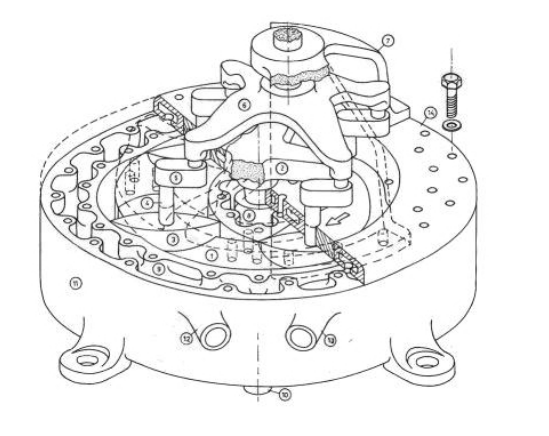
\includegraphics[width=0.5\textwidth]{perspectiva_mrcvc.png}
    \caption{Motor Rotativo de Combustión a Volumen Constante}\label{fig:mrcvc}
\end{figure}

En trabajos anteriores~\parencite{lopez16,lopez13}~se han mencionado
las características que hacen al MRCVC un motor atractivo: la geometría de la
cámara de combustión y del conjunto rotante permiten que gran parte del proceso
de combustión se realice a volumen constante, además de tener un balanceo
mecánico de fuerzas que le permite alcanzar altas velocidades de rotación.
%
Esto promete un funcionamiento más suave del motor, además de una reducción del
ruido y desgaste en comparación a motores rotativos tradicionales (Wankel) y
reciprocantes.
%
Por otro lado hay que mencionar que los motores rotativos traen consigo una
serie de problemas como la necesidad de introducir aceite a la cámara de
combustión para lubricar elementos móviles, el solape de cámaras durante la
apertura de los puertos y en particular al MRCVC un complejo sistema de
sellos~\parencite{roldan}.

%%%%%%%%%%%%%%%%%%%%%%%%%%%%%%%%%%%%%%%%%%%%%%%%%%%

La motivación de este trabajo surge del deseo de continuar con el desarrollo del
MRCVC y mejorar el pre-diseño de los sistemas de intercambio de gases, sentando
la base para una futura optimización de los mismos en un motor con requisitos de
diseño concretos.


Se buscó obtener un pre-diseño satisfactorio del sistema poniendo énfasis en la
geometría de los puertos de admisión y escape, definiendo las métricas a
utilizar para medir la eficiencia del sistema y poder realizar comparaciones
cuantitativas de los diseños propuestos.
%
% El prediseño consiste en definir las métricas a utilizar para medir la
% eficiencia del sistema, rea así como también poder comparar cualitativamente
% y cuantitativamente diferentes geometrías.
%
Debido al costo computacional de las simulaciones necesarias para realizar esta
optimización se restringe el modelado de la geometría a definir posiciones
angulares, largos y diámetros de los puertos.
%
No se repara en detalles como la forma de la transición entre las paredes del
puerto hacia la cámara de combustión, el ángulo al estator y detalles similares.

%%%%%%%%%%%%%%%%%%%%%%%%%%%%%%%%%%%%%%%%%%%%%%%%%%%
La optimización se realizó utilizando en conjunto una serie de herramientas de
simulación, de las cuales las principales fueron:

\begin{enumerate}
        %
    \item ICESym~\parencite{icesym}, simulador de motores de combustión interna basado en modelos cero-/uni-dimensionales (0D/1D).
        %
    \item OpenFOAM~\parencite{openfoam}, la herramienta libre de CFD.
        %
    \item Salome~\parencite{salome}, plataforma libre para simulación numérica.
        %
\end{enumerate}

\nomenclature[F]{\(CFD\)}{\textit{Computational Fluid Dynamics.}}

Se desarrolló un optimizador capaz de generar y evaluar diferentes geometrías
con el fin de buscar una combinación de parámetros que maximicen indicadores de
eficiencia del sistema, como por ejemplo, el rendimiento volumétrico del motor
para un rango de velocidades determinado.

El proceso de optimización consta de una primera aproximación utilizando como
punto de partida los resultados de trabajos anteriores~\parencite{lopez13}, en
los cuales se evaluó el funcionamiento del los parámetros que definen la
geometría de los sistemas de intercambio de gases, en particular: diámetros y
longitudes de conductos y reglaje o posición angular de los puertos.

La optimización se realiza con un algoritmo evolutivo (o genético) funcionando
en conjunto con ICESym, este último provee el puntaje a cada configuración del
motor necesario para estos procesos de optimización.
%
El puntaje se introduce en la función objetivo, la cual evalúa a cada uno de los
candidatos generados por el algoritmo.

El diseño preliminar de la primera ronda de optimización se volcó en un modelo
3D de los puertos, parametrizado de modo tal que se puede alterar rápidamente la
geometría, modificando variables como el diámetro de los conductos y la posición
relativa en la periferia del motor.
%
Este modelo 3D se utilizó para extraer la geometría a simular con OpenFOAM y
realizar flujometrías de las que se obtiene un valor del flujo másico
($\dot{m}$) en estado estacionario para un punto operativo del motor, es decir,
para una combinación de diferencia de presión entre puerto y cámara de
combustión ($\Delta P$) y el grado de apertura del puerto ($l_{v}$).
%
El flujo másico se utilizó para medir la eficiencia con la cual escurre el gas a
través del puerto, por medio del $C_{D}$ con el objetivo de crear un mapa del
coeficiente de descarga que sea función de las variables mencionadas.
%
Este mapa se utiliza como retroalimentación del simulador de motores ICESym,
para tener un mejor modelado del flujo de gas a través de los puertos en un
rango operativo del motor y con esto realizar una nueva corrida de optimización
para refinar el diseño obtenido en la primera iteración.
%
\nomenclature[PO]{\(\dot{m}\)}{Caudal másico}
\nomenclature[F]{\(C_{D}\)}{Coeficiente de descarga}

% Primer capitulo
La organización de este trabajo es como sigue.
%
En el presente capítulo se dio una introducción al trabajo, motivación y
objetivos del mismo.

% Segundo capitulo
En el segundo capítulo se da una breve descripción del funcionamiento de los
motores de combustión interna, seguido de los indicadores utilizados para medir
el rendimiento de motores en general e indicadores particulares de la
eficiencia de los sistemas de intercambio de gases, como el rendimiento
volumétrico y la fracción de gases residuales.
%
Luego, se describe el funcionamiento del MRCVC, indicando los aspectos que
hacen atractivo a este motor, además de desventajas del mismo y las posibles
aplicaciones.
%
También se describe el proceso de intercambio de gases y se define el
coeficiente de descarga $C_D$ y las ecuaciones asociadas.
%
Para finalizar el capítulo se presentan las flujometrías a realizar, modelos de
turbulencia utilizados y las condiciones iniciales y de contorno aplicadas en
las simulaciones.
%

En el tercer capítulo se describe la parte computacional del trabajo, se
presenta el simulador de motores \emph{ICESym}, el optimizador desarrollado y la
integración entre ambos programas.
%
Seguido de una descripción del funcionamiento del optimizador, los motivos de
seleccionar un algoritmo de tipo evolutivo o genético, las ventajas y
desventajas, los componentes básicos y finalmente la implementación del mismo.
%
En este capítulo también se presenta el software utilizado para realizar las
flujometrías, \emph{OpenFOAM}, la implementación de las condiciones iniciales y
de contorno, extracción de datos de ICESym y otras herramientas necesarias para
generar el modelo de CAD del puerto, malla y otros detalles relativos al proceso
de utilizar el programa.

% Cuarto capítulo
En el cuarto capítulo se presenta el desarrollo del trabajo, dando los resultados
de cada etapa.

% Quinto capítulo
Por último, se dan las conclusiones del trabajo, opiniones finales y una
perspectiva a futuro o posibles trabajos a seguir.
